\documentclass{article}
\usepackage[utf8]{inputenc}
\usepackage{hyperref}
\usepackage{algorithm}
\usepackage{algorithmic}
\usepackage{fancyhdr}
\usepackage{graphicx}
\usepackage{listings}
\usepackage[
    backend=biber, 
    natbib=true,
    style=numeric,
    sorting=none
]{biblatex}
\addbibresource{reference.bib}
\usepackage{listings}
\usepackage{xcolor}
\graphicspath{ {./images/} }

%New colors defined below
\definecolor{codegreen}{rgb}{0,0.6,0}
\definecolor{codegray}{rgb}{0.5,0.5,0.5}
\definecolor{codepurple}{rgb}{0.58,0,0.82}
\definecolor{backcolour}{rgb}{0.95,0.95,0.92}

%Code listing style named "mystyle"
\lstdefinestyle{mystyle}{
  backgroundcolor=\color{backcolour},   commentstyle=\color{codegreen},
  keywordstyle=\color{magenta},
  numberstyle=\tiny\color{codegray},
  stringstyle=\color{codepurple},
  basicstyle=\ttfamily\footnotesize,
  breakatwhitespace=false,         
  breaklines=true,                 
  captionpos=b,                    
  keepspaces=true,                 
  numbers=left,                    
  numbersep=5pt,                  
  showspaces=false,                
  showstringspaces=false,
  showtabs=false,                  
  tabsize=2
}

%"mystyle" code listing set
\lstset{style=mystyle}

\pagestyle{fancy}
\fancyhf{}
\rhead{Computer Graphics}
\lhead{CS 440}
\cfoot{\thepage}

\begin{titlepage}
    \begin{center}
        \vspace*{1cm}
            
        \Huge
        \textbf{Visualizing Music: A novel approach to Chord visualization through Computer Graphics Methods}
            
        \vspace{0.5cm}
        \LARGE
        Final Project for \\
        CS 440 - Computer Graphics - L1
            
        \vspace{1.5cm}
            
        \textbf{Syed Ammar Mahdi (03691) \\ Fatima Nadeem (03768) \\ Kabir (03925)}
            
        \vfill
            
        A research report for the final course project of Computer Graphics presented for the degree of\\
        Computer graphics
            
        \vspace{0.8cm}
            
        \Large
        Department Name\\
        University Name\\
        Country\\
        Date
            
    \end{center}
\end{titlepage}

\begin{document}

\tableofcontents
\newpage
\section{Abstract}

The interplay between music and images lends itself to interesting approaches in a computer graphics context. A musical piece can have multiple subjective visual representations, but finding a mapping from sound to image that allows the viewer to infer some musical properties of the music is a daunting task. In this paper we discuss a novel approach to mapping a chord progression in a piece of music to different colours, using some of the techniques that were discussed in CS-440 (namely interpolation). The approach outlined here maps all 12 notes of the western chromatic scale to the 12 colours of the RGB colour wheel, then uses the pre-mapped colours as reference points for chord progressions; each note/colour of the chord is interpolated to visually represent musical intervals. The output is a grid of pixels where each chord is represented as a line of interpolated pixels; this attempts to visually represent the melodic and subjective emotional content of different chords to colours in an image. For the implementation, the myimage class in python was used, which was introduced in the first assignment. The limitations of the approach are also highlighted, as well as possible future improvements to the algorithm.

\section{Introduction}

The primary concern of Computer Graphics is to 'display pretty pictures on a computer'\footnote{Saleem, Waqar. "CS 440: Lecture 1." Habib University, August. 2020}. In a similar vein, the primary concern of music is to perhaps way of arranging aesthetically pleasing sounds together in a meaningful way. Although music and images are both seemingly different domains, as they are based on the different senses of sight and sound respectively, there have nonetheless been countless approaches to convert from one domain to other since at least the time of the ancient Greeks.\footnote{Pythagoras and Aristotle both attempted to correlate musical scales to colours (See [1]).}\\

Human hearing is similar to light in the sense that sounds and light are both logarithmic; The human eye corresponds to changes in brightness on the visible light spectrum in a similar way to how the ear perceives sounds on the decibel scale (i.e. logarithmically). Both light and sound are waves that are picked up by human sensory organs and correspond to a phenomenon in the brain. Just as vision in computer graphics is modelled based on the human eye and visual system (as we saw in the first module of the course), so too can sound be modelled based on the human hearing system and how the brain perceives pitches.\\

The visualization of sounds can be broken down into two major categories; exact representations and abstract mappings. Exact representation of sound has only been possible in modern times, through the use of technology that can accurately visualize the waveform of a sound. Oscilloscopes are a good example of this; through vector graphics displays (or vector graphics simulated on a raster display, as in the case of digital oscilloscopes), they can accurately display the output of sound waves on a screen. This has lead to some interesting visualizations over the years, such as oscilloscope music (see figure below). In such music, the output images are quite literally the sound frequencies being visualized as they are. Software such as Winamp also display interesting colours and visuals based on the frequency of the input sound waveform. Both oscilloscope music and milkdrop are examples of the exact representation approach to visualizing music.

\begin{figure}
    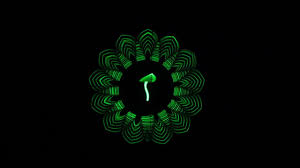
\includegraphics{shrooms.jpg}
    \centering
    \caption{Example of oscilloscope music (Jerrobeam Fenderson, Shrooms\footnote{Original song: https://www.youtube.com/watch?v=19jv0HM92kw}})
    \label{fig:shrooms}
\end{figure}

However, the human brain does not perceive musical notes as individual frequencies of sound, but in relation to one another. The exact representation approach, therefore, fails to capture the harmonic, rhythmic and melodic qualities of music in a meaningful way. This is where the abstract representation approach shines, where one assigns a set of rules to map musical tones to output images. It is this approach that we have considered in our method of visualizing chords progressions.

\section{Literature Review}
This section is dedicated to discussing the different research works that were researched as part of this project. Firstly, the main paper that guided our implementation as well as provided the impetus for it is discussed. Following that, the section goes into other helpful and related works.

\subsection{Main Work Regarding Image to Sound Conversion}
The paper in question here is \cite{margounakis2006converting}. The paper basically dives into the problem by providing a mapping between image and sound characteristics. It uses this mapping to launch some concepts such as chromatic bricks and segments that make up a particular image while also specifying the notes for a melodic composition as well. The paper and its methodology served as a direct inspiration for the one developed for this project and focused on aspects it discussed, i.e. representing musical notes as visual 'blocks' that are assigned a specific RGB value based on a set of rules. The idea of a 'mapping matrix' introduced in the paper was also relevant for us to determine which features to consider in our output pixel grid; however instead of the one shown by the authors, we used a different subjective mapping matrix that only mapped pitch and pitch relations (i.e. intervals) in the 'Sound' domain to brightness and colour in the 'Image' space.

\subsection{Other Relevant Work}
The further work of the researchers of the above discussed work also gave a direction for where their work was headed. In \cite{politis2008image}, they stretch the idea further to incorporate a reversal of the main problem and devise an effective way to generate imagery from sound given. This method also further utilizes the concept of chromaticism in music; the idea of assigning colour to sound for the human psycho-acoustic domain. Furthermore, this paper also researched how the synthesis of sound and imagery could greatly benefit a visual performance and promote a cross cultural appreciation of sound and imagery. \\

\cite{ciuha2010visualization} proved as yet another inspiration for our implementation, as it highlighted a direct approach to how colours can be mapped to sound using the circle of fifth; an important concept of music. The modular structure of the circle of fifths directly inspired the idea of mapping the chromatic scale to the colour wheel, and interpolating between those colours in chord progressions.

\section{Our Method}

Our approach is a novel one in colour representations of a specific element of a musical piece; namely chord progressions. The idea is to take the chord progression in a piece of music, find out the notes in the relevant chord and the colour each note is mapped to, then interpolate between the colours of the chord/notes. This will then display a line of interpolated pixels in the output pixel grid image. The details of this method are elucidated in the sections below.

\subsection{Music Theoretical Background}

A piece of music has several complex elements, such as melody, rhythm, time signature and harmony, just to name a few. For the purposes of this study, we restrict the scope of our analysis just to chords alone, which often provide a 'backbone' for the melody of the music being sung or played.\\

The musical background needed to understand our approach of mapping chords to colours are the concepts of \textbf{notes}, \textbf{scales}, \textbf{intervals}, \textbf{semitones} and \textbf{chords}.\\

\textbf{Notes} are simply pure frequencies of sound played that sound good in relation to one another. For example, the 'middle C note' has a frequency of ~261.63 Hz, while the standard A4 note has a frequency of 440 Hz.\\

\textbf{Scales} are simply sets of notes that have been defined according to rules that predefined the distance between the previous note and the next note in the set. The most common scales in western music are the major scale and the minor scale. Examples include the C major scale {C, D, E, F, G, A, B} and the A minor scale {A, B, C, D, E, F, G}; both of which are simply the white keys on the piano starting from the C note and A note, respectively.\\

\textbf{Intervals} are the distance between two notes and define the notes' musical relationship to one another. For example, the interval of a fifth is the distance between the 1st and the fifth note of a scale.\\

\textbf{Semitones} are the smallest possible distance between a two notes, corresponding to each 'next' key on a piano or 1 fret on a guitar.\\

Finally, \textbf{chords} are simply groups of notes played together at once. A chord can consist of 2, 3, 4, 5 or more different notes played in unison. Most popular music uses what are known as 'triads' (i.e. or chords with 3 notes played together).

\subsubsection{The Mapping}

In the western musical systems, the complete set of possible notes is known as the chromatic scale. The notes in the chromatic scales are as follows:

\begin{center}
    \{A, A\#/Bb, B, C, C\#/Db, D, D\#/Eb, E, F, F\#/Gb, G, G\#/Ab\}
\end{center}

This can be much more easily visualized using the keys on a piano as detailed in figure\footnote{source: https://www.piano-keyboard-guide.com/wp-content/uploads/2015/04/piano-chromatic-scale.jpg} 2.\\

\begin{figure}
    \centering
    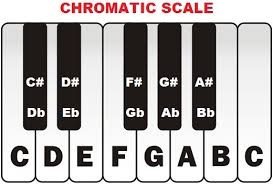
\includegraphics{chromatic.jpg}
    \caption{The western chromatic scale.}
    \label{fig:chroma}
\end{figure}

The X\#/Yb notes above (where {X, Y} represent any of the musical notes) are what are known as 'accidentals', or the black keys on the piano. Here we will use the 'sharp' (X\#) representation of an accidental, for simplicity's sake.\\

The chromatic scale has a modular structure; that means that the note C will be the next note after G\#, just an octave above the previous C note.\\

The RGB colour wheel in its most common representation has 12 colours, as detailed in the figure\footnote{source: https://i.pinimg.com/originals/ad/4b/cf/ad4bcfcd6b94b8be1aaa9717c08ff580.png} 3.

\begin{figure}
    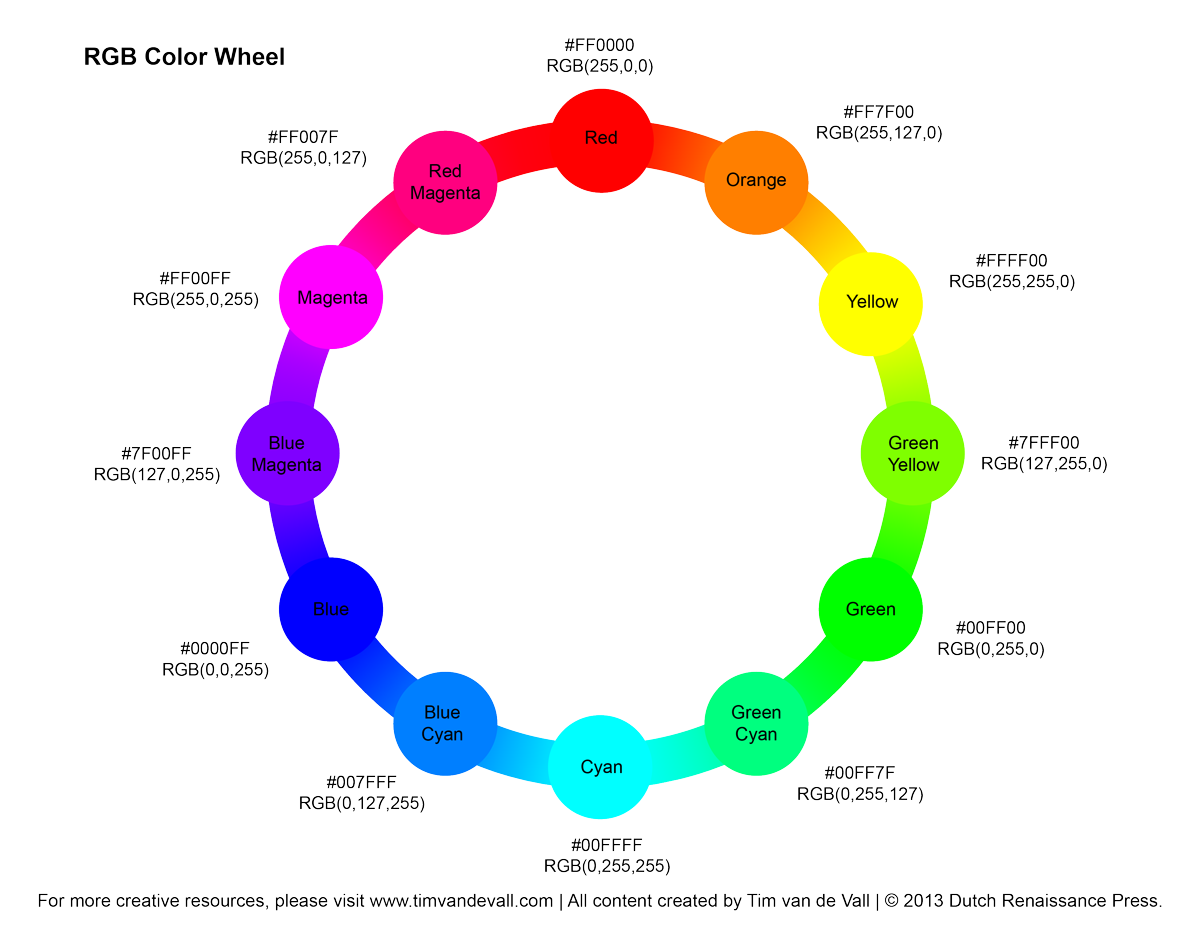
\includegraphics[scale=0.3]{wheel.png}
    \caption{A commonly used representation of the RGB colour wheel with its respective RGB values.}
    \label{fig:wheel}
    \centering
\end{figure}

One can then imagine a simple mapping between the 12 notes in the chromatic scale and the 12 colours on the colour wheel. Using this as our starting point, we can move on to colour representation of chords from the mapping defined above, which will then interpolate the colours in the chord depending on the notes.

\subsection{Resources}

Python was used as the coding language for implementing the algorithm. Although certainly possible, there is no library used for approximating chord progression information automatically from a given musical file \footnote{Although undoubtedly cool, this would be excessive as chord progressions for nearly any musical piece on the planet already exist and are a simple click away.}. The python imaging library (PIL) is used, with its implementation of a myimage class, to output the chord progressions as a coloured grid of interpolated pixels.

\section{Code}

The main code of our program is included in the listing below. The procedure, which was briefly summarized before, is explained in detail in the code file and its comments.

\lstinputlisting[language=python, 
caption= Main Code for Sound To Image Conversion
]{music.py}
\section{Output}

The output of our code is displayed in Figure 4.\\

\begin{figure}
    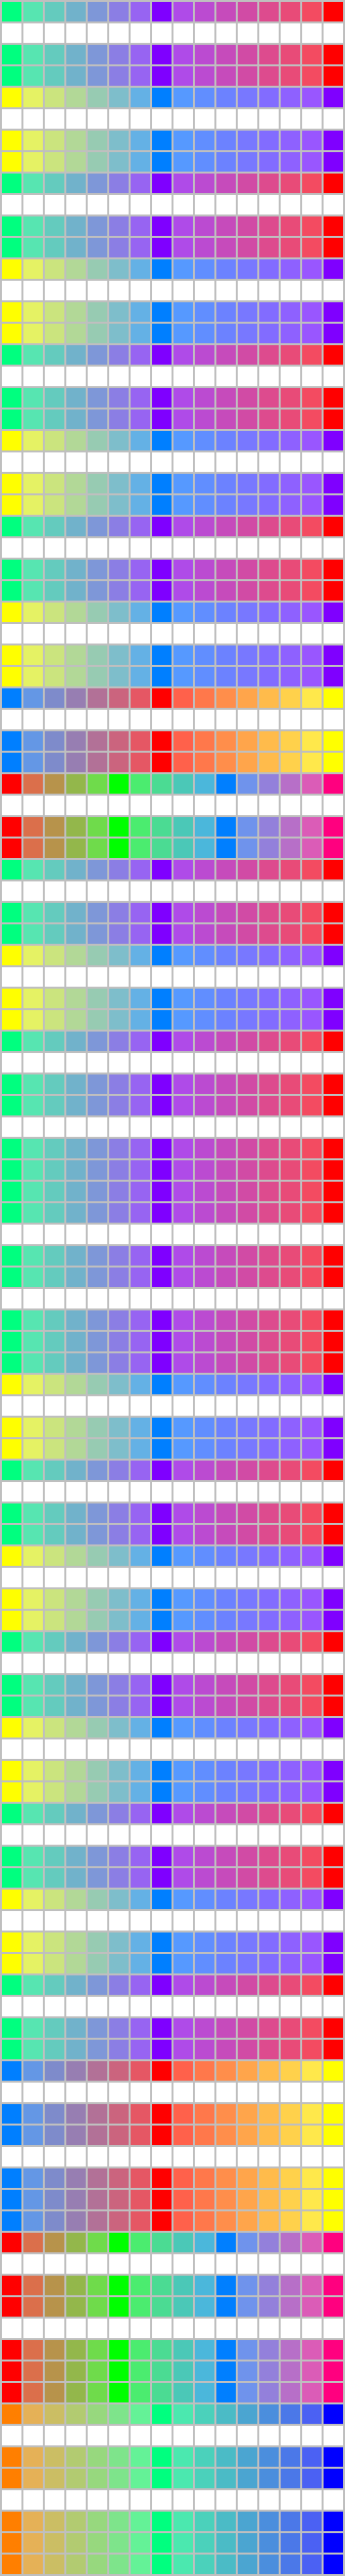
\includegraphics[width=0.2\linewidth]{output.png}
    \centering
    \caption{The chromatic wall produced as an output of the chord progression.}
    \label{fig:output}
\end{figure}

The output is an instance of the 'MyImage' class with large virtual pixels for easier visualization of chords. Each column in the output image is $\frac{1}{16}$th a complete musical beat, and each row represents either a chord (represented by interpolated colours) or silent beats (represented by a white line). Therefore, just as the musical piece progresses beat by beat so too must one iterate over each row of the output image to visualize the musical piece.\\

The piece being played in question is the first verse of the song in appendix A, with the relevant chord progressions provided. The output shown here is only for the first verse of the song.

\section{Results}

The interpolated colours in the output image for each chord assign an emotional 'feel' to each chord that is being played based on their intervals. For example, triads consist of 3 musical intervals, whereas seventh chords consist of 4 musical intervals; seventh chords are, therefore, musically 'richer' than triads and have a wider range of colours being interpolated between them in comparison to triads.\\

Different chord progressions for different musical pieces would yield different interpolated colours, and can vary vastly to the one shown in the output image. What stays constant, however, is the degree to which musical notes are interpolated based on intervals; an E major chord will have a different colour representation with our approach than a D major chord, but the relative degree to which the colours are interpolated in relation to one another will remain constant.\\

Though the question of asking what colour a chord is perhaps similar to asking what the colour blue smells like, the approach highlighted here nonetheless provides one meaningful way to assigning colours to chords based on their intervals. The abstract representation approach at its core is a subjective colour representation of music, just as the phenomenon of sound and sight are 'happenings' in our brain. Nonetheless, the core harmonic structure of the chord progression remains intact even after the colour mapping, which gives some meaningful visual representation to a non-visual phenomenon.\\

\subsection{Applications}

Other than simply looking pretty, the approach highlighted here could provide an alternate way to synchronize music with colour. As an example, one can imagine how electronic music festivals have colours being displayed with the music being played. Although most of these colours shifts occurs either through random techniques such as pseudo-random noise perturbations, or in relation to the rhythm and loudness of the music being played, the method detailed here could provide a useful novel approach to visualizing music based on its underlying musical properties.\\

Unfortunately the model we have used is too simple to provide an alternate visual representation of music, as it lacks some of the major important elements of music as whole (detailed further in the section below) and thus cannot be inverted to produce the original musical piece back from the outputted image. However, if fleshed out further, it is perhaps not too far-fetched to consider this as a more appealing alternative to traditional musical notation systems, none which are currently not too visually appealing.\footnote{Most guitarists dread traditional sheet music, not because it is complex but because it is a bore to look at and therefore a threat to the 'cool-guy' guitarist image.}\\

\subsection{Limitations and Future improvements}

Chord progressions do not exist on their own as single beats of a chord or silence, but also require additional information to be played properly: the time duration for which a chord is played. This is not taken into account in our model, but can easily be modelled by making the array of notes in the code a 2D-array, with each array element A[m][1] representing the duration of time for which a note is played (1, 2, $\frac{1}{2}$, $\frac{1}{4}$, $\frac{1}{16}$, and so on). Taking this into account would have the effect of changing the length of each chord-pixel-row in the output image based on the duration for which it must be played.\\

There is also no way to tell the time signature of the music using this approach; the viewer does not know simply by looking at the output image, for example, if there are 8 beats per measure, 16 beats or even an eccentric number like 5 beats. This can be remedied by specifying a separate function argument in the CreateWall function specifying the time signature of the music, and adding a counter variable that increments with each iteration of the loop which lets the program know if one complete measure has passed or not. Further still, each row of the output image could be rearranged to instead represent one complete measure per row instead of one beat, to make it easier to visualize when a measure has completed. This would not only compact the outputted pixel grid greatly, but also lend itself better for the purposes of developing a visual musical colour notation.\\

Furthermore, from a computational perspective, one can consider a efficient data structure more better for storing musical elements, just as face-based data structures lend themselves better to representing graphical information. If note duration is also modelled along with note pitch in our 2D arrays, the program would have a complexity of $\mathcal{O}(n^2)$, which could grow cumbersome for large musical pieces (consider that the output shown in our image for a flat list representation is only enough to represent the first 30 seconds of a song). Although not formally explored yet, the circular queue/ring data structure hold some promise of a possible direction of future exploration, as it lends itself better to the idea of musical measures and has a more intuitive representation for certain elements of music which are modular (i.e. The circle of fifths, octaves).

Additionally, the scope of music that we have modelled is quite limited from a musical theory perspective, as there are hundreds of chords and scales/modes not coded in the program. Surprisingly, this does not have much of an effect for most modern music; almost 95\% of all pop music uses the same four major/minor chords, and rock music utilizes fifth and seven chords frequently, which have been included in our program.\footnote{This is why by learning just 8 chords on the guitar, one can effectively play hundreds of thousands of popular songs.}\\

Finally, although the chords are assigned colours based on their intervals, there is still no way to distinguish between different types of triads or other chords. The old musical truism, "Major chords are happy, minor chords are sad" had no way of showing in our model, as the colours between the two chords are interpolated in the same way. This can be remedied through several improvements to the chord colour mapping model; interpolating based on scale degrees rather than standardized distances and considering the colours of chords in relation to one other (the previous chord that came before it\footnote{A B minor chord followed by a D major chord sounds very different to a D major chord followed by a B minor chord; try it!}) rather than in isolation, and assigning colours based on a vector model from the distance and angle on the circle of fifths between subsequent chords\footnote{See \cite{ciuha2010visualization} for a detailed explanation on the vector model of musical relationships, which is a much better mapping method compared to the one we have used as it preserves musical structure much more naturally} rather than direct mapping of the chromatic scale to the RGB wheel are some of the methods that we can use to better preserve and visualize musical structure in our colour interpolation method.\\

\section{Conclusion}

To summarize, in our research report we have explained why an abstract mapping of a musical piece to visual output is a superior approach to an exact visual representation of sound. We have then highlighted some of the salient features of music and how they can be represented visually, and have used a computer graphics method and an image class used in our course to develop an entirely new approach\footnote{As far as we know} to visualizing musical elements through colour interpolation of the chord notes. Finally, we have discussed the major limitations of our method, as well as highlighted further ways of improving our model and future directions of research to make it a more musically sound visualization. In doing so we hoped to have ventured into relatively uncharted territory by syncretizing the domain of computer graphics with music; an area with relatively little research conducted into it to this date.

\section{Appendix A: Penalize}

The following is a parody of the song "Still Alive"\footnote{source: https://www.youtube.com/watch?v=Y6ljFaKRTrI} from the video game portal, which will be used as an example song to output chord colours using our program.

The song is written in guitar chord notation and has been adapted from the following source: https://tabs.ultimate-guitar.com/tab/misc-computer-games/portal-still-alive-chords-588968

\begin{verbatim}
[VERSE]

D Bm D Bm
D Bm D Bm
Em A7
D Bm D Bm
D Bm D Bm
D Bm D Bm
Em A7
A#7

[CHORUS]

F C A# F
F C A# F
Gm C F C Dm
A# A7

D Bm D Bm
D Bm D Bm

[Intro/Verse 1]

             D     Bm D
This was not tender
    Bm           D
I'm making a note here
Bm           D Bm
'What a mess'
     Em              A7        D      Bm D
Your code comments are against my satisfaction

Bm         D     Bm D
'Horrible render'
Bm             D       Bm      D Bm
we do what we must because we can
Em                   A7                   A#
It's for the good of all of us Except the ones who have dropped


[Chorus]

            F        C           A       F
but there's no sense crying over every mistake
         F       C                A#         F
I commend you for trying but that’s not what it takes
        Gm           C            F      C  Dm
I’m on top of this course and I’ll show you no remorse
        A#           A7
When I’m gonna penalize


D Bm D Bm
D Bm D Bm


[Verse 2]

             D    Bm  D
I'm not even angry
Bm          D      Bm      D   Bm
I'm being so sincere right now
Em              A7                     D   Bm D
I wish I could erase your code from memory
    Bm           D   Bm D
And tear it to pieces
    Bm               D   Bm      D  Bm
And throw every piece into a fire
Em                 A7                    A#
As it burns I hope you learn how to write decent code


[Chorus]

          F         C           A#        F
Now these pixels on the screen make a beautiful line
          F         C           A#         F
It’s a shame your program did not render on time
        A#          C                F       C       Dm
You may think it’s no fun, but think of all the things you’ll learn
        A#           A7
When I am gonna penalize

D Bm D Bm
D Bm D


[Verse 3]

               D  Bm  D
Go ahead and contest
  Bm            D      Bm      D   Bm
I think the instructor will take my side
Em                A7                  D   Bm D
Maybe you'll find someone else to help you
Bm           D   Bm D
Maybe Anisa?
Bm              D     Bm            D  Bm
That was a joke - haha - FAT CHANCE!
Em           A7                         Bb
Anyway, your tears are great - they're so delicious and moust


[Chorus]

        F         C                    A#         F
Look at me still talking while there are more reviews to do

      F        C                  A#           F
When I read your gibberish it makes me GlaD I’m not you
       A#         C                F       C       Dm
There’s no reason to be mad; Your code’s honestly not half-bad
       A#          A7            D
But I am still gonna penalize


[Outro]

Bm      D           Bm           D
And believe me, I will penalize!
Bm        D             Bm            D
And for no reason I will penalize
Bm        D             Bm           D
I feel FANTASTIC when I penalize!
Bm              D           Bm            D
And for no reason I will penalize!
Bm              D            Bm           D
And if your code runs I'll still penalize!
Bm      D
Penalize
Bm      D 
Penalize
\end{verbatim}

\printbibliography

\end{document}
